\section{Aufbau und Durchführung}
\label{sec:Durchführung}
Zunächst wird die Funktionsweise des Signal Processors bzw. Lock-In Amplifier des Lock-In-Verstärkers betrachtet.
Dabei wird die Spannungsamplituden der Ausgänge Reference und Oscillator
auf Variation bzw. Konstanz mittels eines angeschlossenen digitalen Oszillators hin
überprüft. Der konstante Amplitudenwert wird notiert.
Anschließend ist die Schaltung, welche in Abbildung \ref{fig:aufbau1} zu sehen ist, schrittweise aufzubauen, wobei der Noise Generator für diesen
Teil ersteinmal überbrückt wird. Zuerst wird nur ein sinusförmiges Eingangssignal $U_\text{sig}$ mit einer Frequenz von 1 kHz und einer Spannung von 10 mV auf den
Verstärker gegeben und danach mit einer ebenfalls sinusförmigen Referenzspannung $U_\text{ref}$, gleicher Frequenz, gemischt. Das resultierende Signal wird auf dem digitalen Oszilloskop
ausgegeben. Für fünf verschiedene Phasen der Referenzspannung, welche am Reference Ausgang einstellbar ist, wird eine Grafik erstellt.
Anschließend wird die Schaltung, wie in Abbildung \ref{fig:aufbau1}, vollständig nachgebaut, wobei der Noise Generator weiterhin überbrückt wird.
Nun wird wieder das Ausgangssignal betrachtet, welches nun allerdings integriert wird, das heißt mit Nutzung des angeschlossenen Tiefpasses. In diesem Aufbau werden verschiedene Ausgangsspannungen 
in Abhängigkeit von der Phasenverschiebung der Referenzspannung aufgenommen, welche wieder am Reference Ausgang verändert wird.
In einem nächsten Schritt wird der Noise Generator wie in Abbildung \ref{fig:aufbau1} angeschlossen. Zu Beachten ist, dass sich die vom Noise Generator erzeugten Rauschsignale in der
selben Größenordnung befinden wie die Signalspannung $U_\text{sig}$. Wie schon zuvor wird nun wieder die Ausgangspannung $U_\text{out}$ in Abhängigkeit der Phasenverschiebung aufgenommen.
\begin{figure}
  \centering
  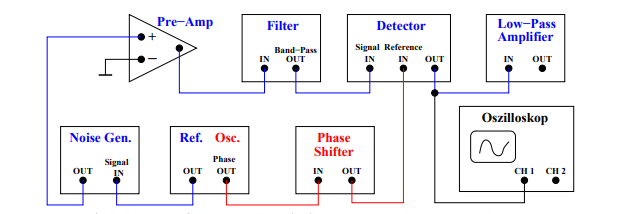
\includegraphics{content/abbildung2.png}
  \caption{Schaltskizze zur Messung der Ausgangspannung in Abhängigkeit zur Phasenverschiebung \cite[4]{V303}}
  \label{fig:aufbau1}
\end{figure}
In einem letzten Schritt ist der Lock-In-Verstärker auf die Rauschunterdrückung hin zu untersuchen.
Hierzu wird, wie in Abbildung \ref{fig:aufbau2} dargestellt, die Schaltung modifiziert, so dass nun statt des Noise Generators eine LED und eine Photodiode geschaltet sind, welche einen Abstand $r$ von einander haben.
Zu Beachten ist, dass die LED mit einer Rechteckspannung versorgt wird, welche im Frequenzbereich von 50 Hz bis 500 Hz
liegt, weshalb hier mit einer 300 Hz Rechteckspannung gearbeitet wird. Es wird die Lichtintensität der LED in Abhängigkeit des veränderlichen Abstandes $r$ gemessen und notiert. Außerdem ist der maximale Abstand 
$r_\text{max}$ zu bestimmen, an dem das Licht der LED noch mit der Photodiode nachgewiesen werden kann.
\begin{figure}
  \centering
  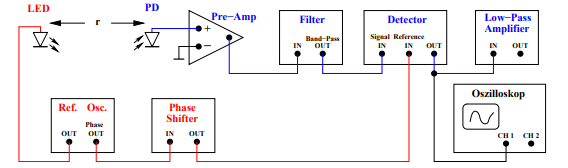
\includegraphics{content/abbildung3.png}
  \caption{Schaltskizze zur Überprüfung der Rauschunterdrückung des Lock-In-Verstärkers mittels einer Photodiode \cite[5]{V303}}
  \label{fig:aufbau2}
\end{figure}